\section{Punto de Vista de Principios}
El punto de vista de principios permite al arquitecto crear una descripción detallada de los principios relacionados con un objetivo ou objetivos específicos de la organización, con el fin de proyectar los valores que propulsan el desarrollo de estos objetivos estratégicos.

\subsection{Modelo de Principios}
\begin{figure}[h]
	\centering
	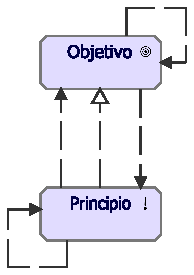
\includegraphics[width=0.3\linewidth]{imgs/modelo/Principios}
	\caption{Modelo Principios}
\end{figure}

Los elementos del modelo de principios permiten transmitir la relación univoca o biunívoca que hay entre los principios de la organización o empresa y los objetivos de la misma. Es una guía del diseño arquitectural de los principios corporativos que se aplican al prestar los servicios de la empresa por medio de valoraciones. Un principio representa una declaración cualitativa de intenciones que la arquitectura debe cumplir.

%\newpage

\subsection{Caso  de Principios}
\begin{figure}[h]
	\centering
	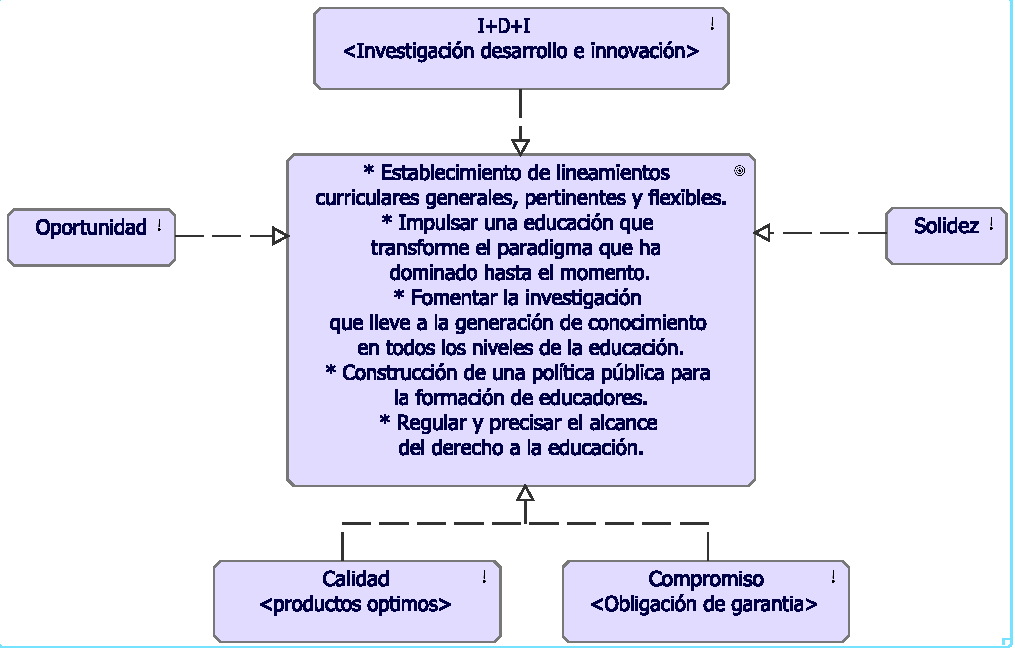
\includegraphics[width=1.0\linewidth]{imgs/motivacion/principios/principios}
	\caption{Caso Principios}
\end{figure}

Los principios que cualifican los objetivos corporativos relacionados con la calidad de la educación son aquellos que permiten el avance de forma asertada de lo que tiene que ver con el enfoque del fomento de investigaciones e impulso a la educación a un nivel mas alto, entre ellos tenemos la investigación desarrollo e innovación, calidad y compromiso.

%\newpage

\subsection{Caso  de Principios}
\begin{figure}[h]
	\centering
	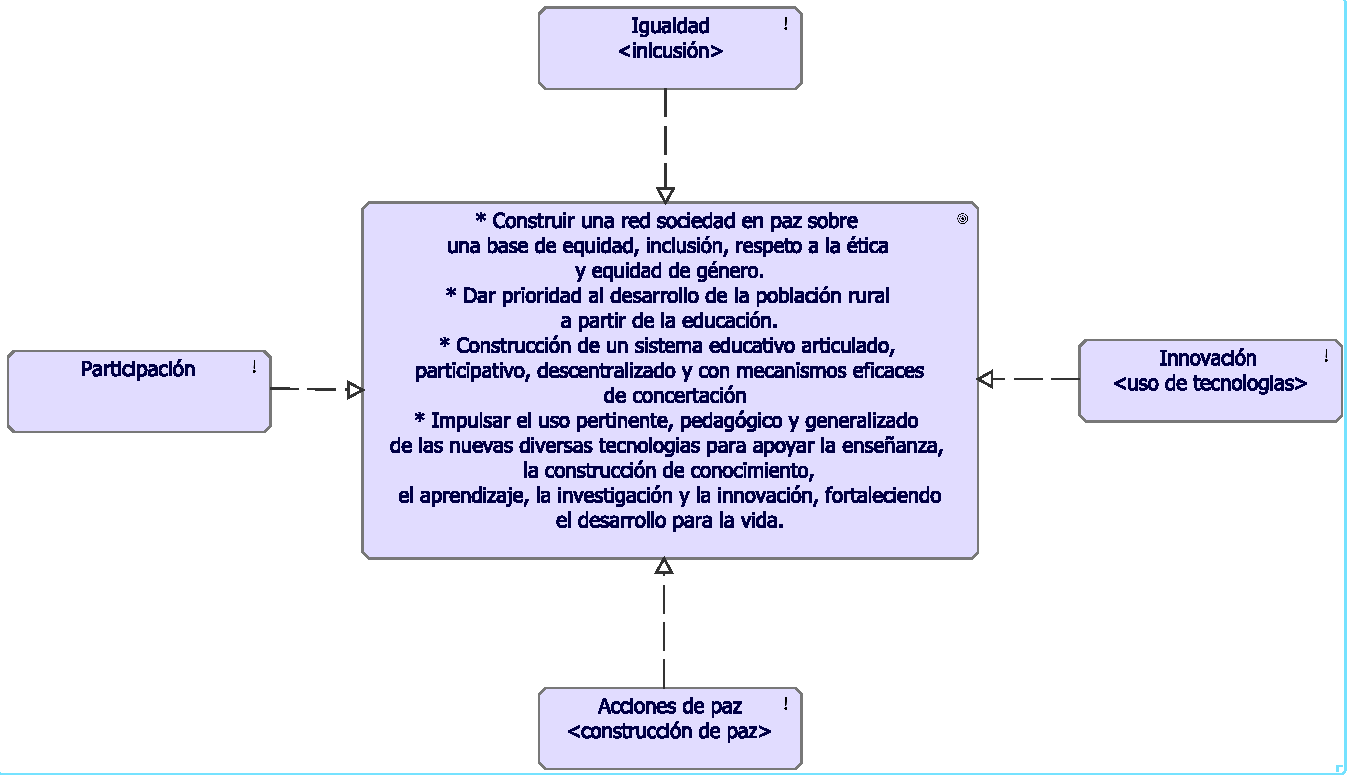
\includegraphics[width=1.0\linewidth]{imgs/motivacion/principios/principios_2}
	\caption{Caso Principios}
\end{figure}

Para construir la paz en nuestro país por medio de la educación que propone el MEN, se logra por medio de los principios que son base esencial para encontrar un equilibrio en la sociedad que potencie la entidad humana como se presentan en ek punto de vista de principios, entre ellos se tiene igualdad, participación, acciones de paz e innovación.